

\section{Wirtschaftliche Gesamtbetrachtung und Rentabilität}

Um die Entscheidung für die Implementierung des neuen Systems fundiert zu begründen, werden in diesem Kapitel die Kosten des bisherigen Ausgangszustands den anfallenden Investitionen und Einsparungen des intelligenten Fehlersupports gegenübergestellt.

\subsection{Rahmenbedingungen und Annahmen}

Die Berechnung basiert auf einer typischen Produktionslinie im Zweischichtbetrieb mit folgenden Parametern:
\begin{itemize}
    \item \textbf{Betriebsdaten:} 220 Arbeitstage/Jahr, 3 Störungen/Tag $\implies$ \textbf{660 Fehlerfälle pro Jahr}.
    \item \textbf{Zeitersparnis durch Intelligenten Fehlersupport:} Reduzierung der Fehlersuchzeit um $10\,\text{Minuten}$ pro Störung (von 25 auf 15 Minuten).
    \item \textbf{Kostensätze:} Maschinenstundensatz $4{,}00\,\text{€/min}$ ($240\,\text{€/h}$); Instandhaltungspersonal $1{,}00\,\text{€/min}$ ($60\,\text{€/h}$).
    \item \textbf{KI-Token \& Daten:} Ringpuffer von $33.400\,\text{Zeichen}$ ($\approx 8.350\,\text{Input-Token}$) + Antwort von $560\,\text{Zeichen}$ ($\approx 140\,\text{Output-Token}$). 
    
    Preis: $\$3{,}00$ / Mio. Input-, $\$5{,}00$ / Mio. Output-Token:
    
    $\frac{8.350 \times \$3{,}00 + 140 \times \$5{,}00}{1.000.000} = \$0{,}02575 \approx \mathbf{\$0{,}03\,\text{bzw. } 0{,}03\,\text{€}}$ pro Fehlerfall.




    \item \textbf{Hardware \& Energie:} Computer im Dauerbetrieb ($15\,\text{W}$) bei $0{,}20\,\text{€/kWh}$.
\end{itemize}

\subsection{Laufende Betriebskosten}

Die laufenden Betriebskosten umfassen vor allem die variablen API-Tokengebühren für die Künstliche Intelligenz, sowie die Stromkosten der verwendeten Hardware:

\begin{itemize}
    \item \textbf{API-Tokenkosten:} $\$0{,}0258$ ($\approx 0{,}0237\,\text{€}$) pro Fehlerfall $\implies$ \textbf{$15{,}67\,\text{€/Jahr}$} bei 660 Aufrufen.
    \item \textbf{Energiekosten:} $15\,\text{W} \times 24\,\text{h} \times 365\,\text{Tage} = 131{,}4\,\text{kWh/Jahr} \implies \mathbf{26{,}28\,\text{€/Jahr}}$.
\end{itemize}

Die gesamten laufenden Betriebskosten betragen also: $15{,}67\,\text{€} + 26{,}28\,\text{€} = \mathbf{41{,}95\,\text{€/Jahr}}$.


\subsection{Erwartete Ersparnisse}

Demgegenüber steht der monetäre Jahresnutzen durch die Reduzierung der Stillstands- und Fehlersuchzeiten um kumuliert $6.600\,\text{Minuten/Jahr}$ ($110\,\text{Stunden}$):
\begin{align}
    \text{Ersparnis}_{\text{Produktion}} &= 6.600\,\text{min} \times 4{,}00\,\text{€/min} = 26.400{,}00\,\text{€/Jahr} \\
    \text{Ersparnis}_{\text{Personal}} &= 6.600\,\text{min} \times 1{,}00\,\text{€/min} = 6.600{,}00\,\text{€/Jahr}
\end{align}

Der Bruttonutzen beträgt somit $33.000{,}00\,\text{€/Jahr}$. Abzüglich der laufenden Betriebskosten ergibt sich eine Jahresersparnis von gesamt  $32.958{,}05\,\text{€}$.

\subsection{Investitionsaufwand}

Bevor von dieser Ersparnis profitiert werden kann, muss das System aber erst Implementiert werden. Für die Erstimplementierung fallen zunächst einmalige Investitionskosten an:

\begin{enumerate}
    \item \textbf{Hardwarebeschaffung:} Industrietauglicher Computer mit GPU: $1.500{,}00\,\text{€}$.
    \item \textbf{Engineering \& Integration:} Programmierung von SPS-Puffer, OPC-UA Gateway, HMI-Anbindung ($40\,\text{h}$ à $75\,\text{€/h}$): $3.000{,}00\,\text{€}$.
\end{enumerate}

\noindent Die einmalige Gesamtinvestition beträgt somit $\mathbf{ 4.500{,}00\,\text{€}}$.

\subsection{Amortisation}

Die Amortisationsdauer dieser Investition berechnet sich aus dem Verhältnis der einmaligen Investition zur jährlichen Ersparnis:
\[
    T_{\text{amort}} = \frac{\text{Investitionskosten}}{\text{Netto-Ersparnis}_{\text{Jahr}}} = \frac{4.500{,}00\,\text{€}}{32.958{,}05\,\text{€/Jahr}} \approx 0{,}137\,\text{Jahre} \approx \mathbf{1{,}6\,\text{Monate}}
\]

Bei der angenommenen Störungsfrequenz von 3 Störungen am Tag refinanziert sich das System bereits nach ca. 90 behobenen Fehlern vollständig. Somit ist dieses System eine sichere Investition. 

Folgende Grafik vergleicht die Kosten durch die Implementierung mit den Kosten, wenn die Implementierung nicht durchgeführt wird.

\begin{figure}[H]
        \centering
        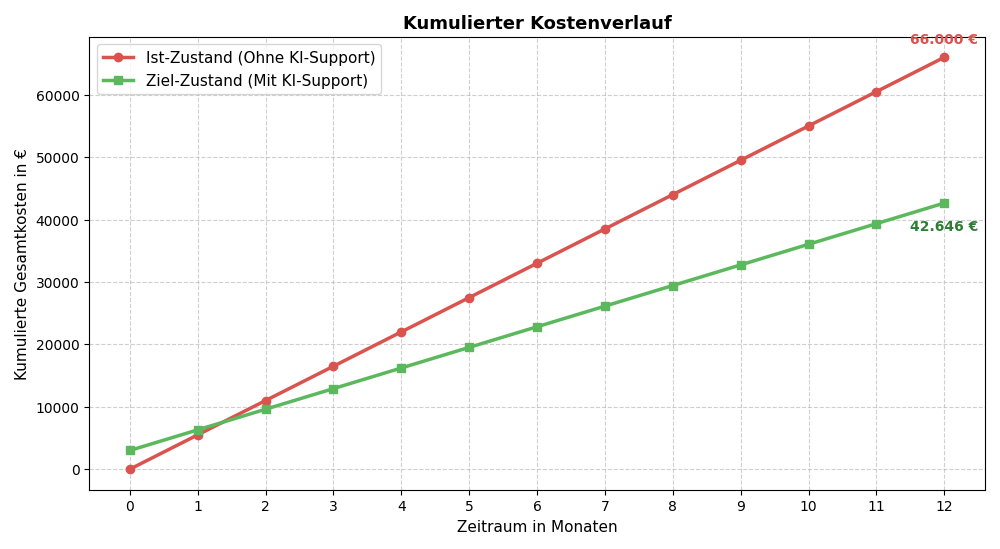
\includegraphics[width=\textwidth]{content/Code_um_Diagramme_darzustellen/Figure_1.png}
        \caption{Vergleich der Kostenentwicklungen bei Implementierung oder Belassen im Ausgangszustand}
        
        \end{figure}

\subsection{Fazit}
Mit einmaligen Investitionen von $4.500\,\text{€}$ und vernachlässigbaren Betriebskosten von unter $42\,\text{€/Jahr}$ weist das Konzept eine extrem kurze Amortisationszeit von unter zwei Monaten auf. Ab dem zweiten Betriebsmonat erwirtschaftet das System einen Netto-Vorteil von rund $33.000\,\text{€}$ pro Anlage und Jahr. Eine Umsetzung wird aus betriebswirtschaftlicher Sicht uneingeschränkt empfohlen.